\documentclass[a4paper,12pt]{article}
\usepackage{amsmath}
\usepackage{graphicx}
\usepackage{float}
\title{Computerized Simulation \\
Exercise No. 3}
\author{name : Seyed Mohammad Ghoreishy \\ teacher : Seyed Amirhossein Tabatabaei }
\date{Date: 1403.09.26}
\begin{document}
\maketitle
\tableofcontents 
\newpage

\section{Exercise 1}
Write a program using the \textbf{accept-reject method} to generate random numbers following a custom probability distribution defined by the piecewise function as follows:
\begin{equation*}
    f(x) = \begin{cases} 
    2x & 0 \leq x \leq 0.5 \\
    2(1 - x) & 0.5 < x \leq 1.
    \end{cases}
\end{equation*}
\begin{figure}[h!]
    \centering
    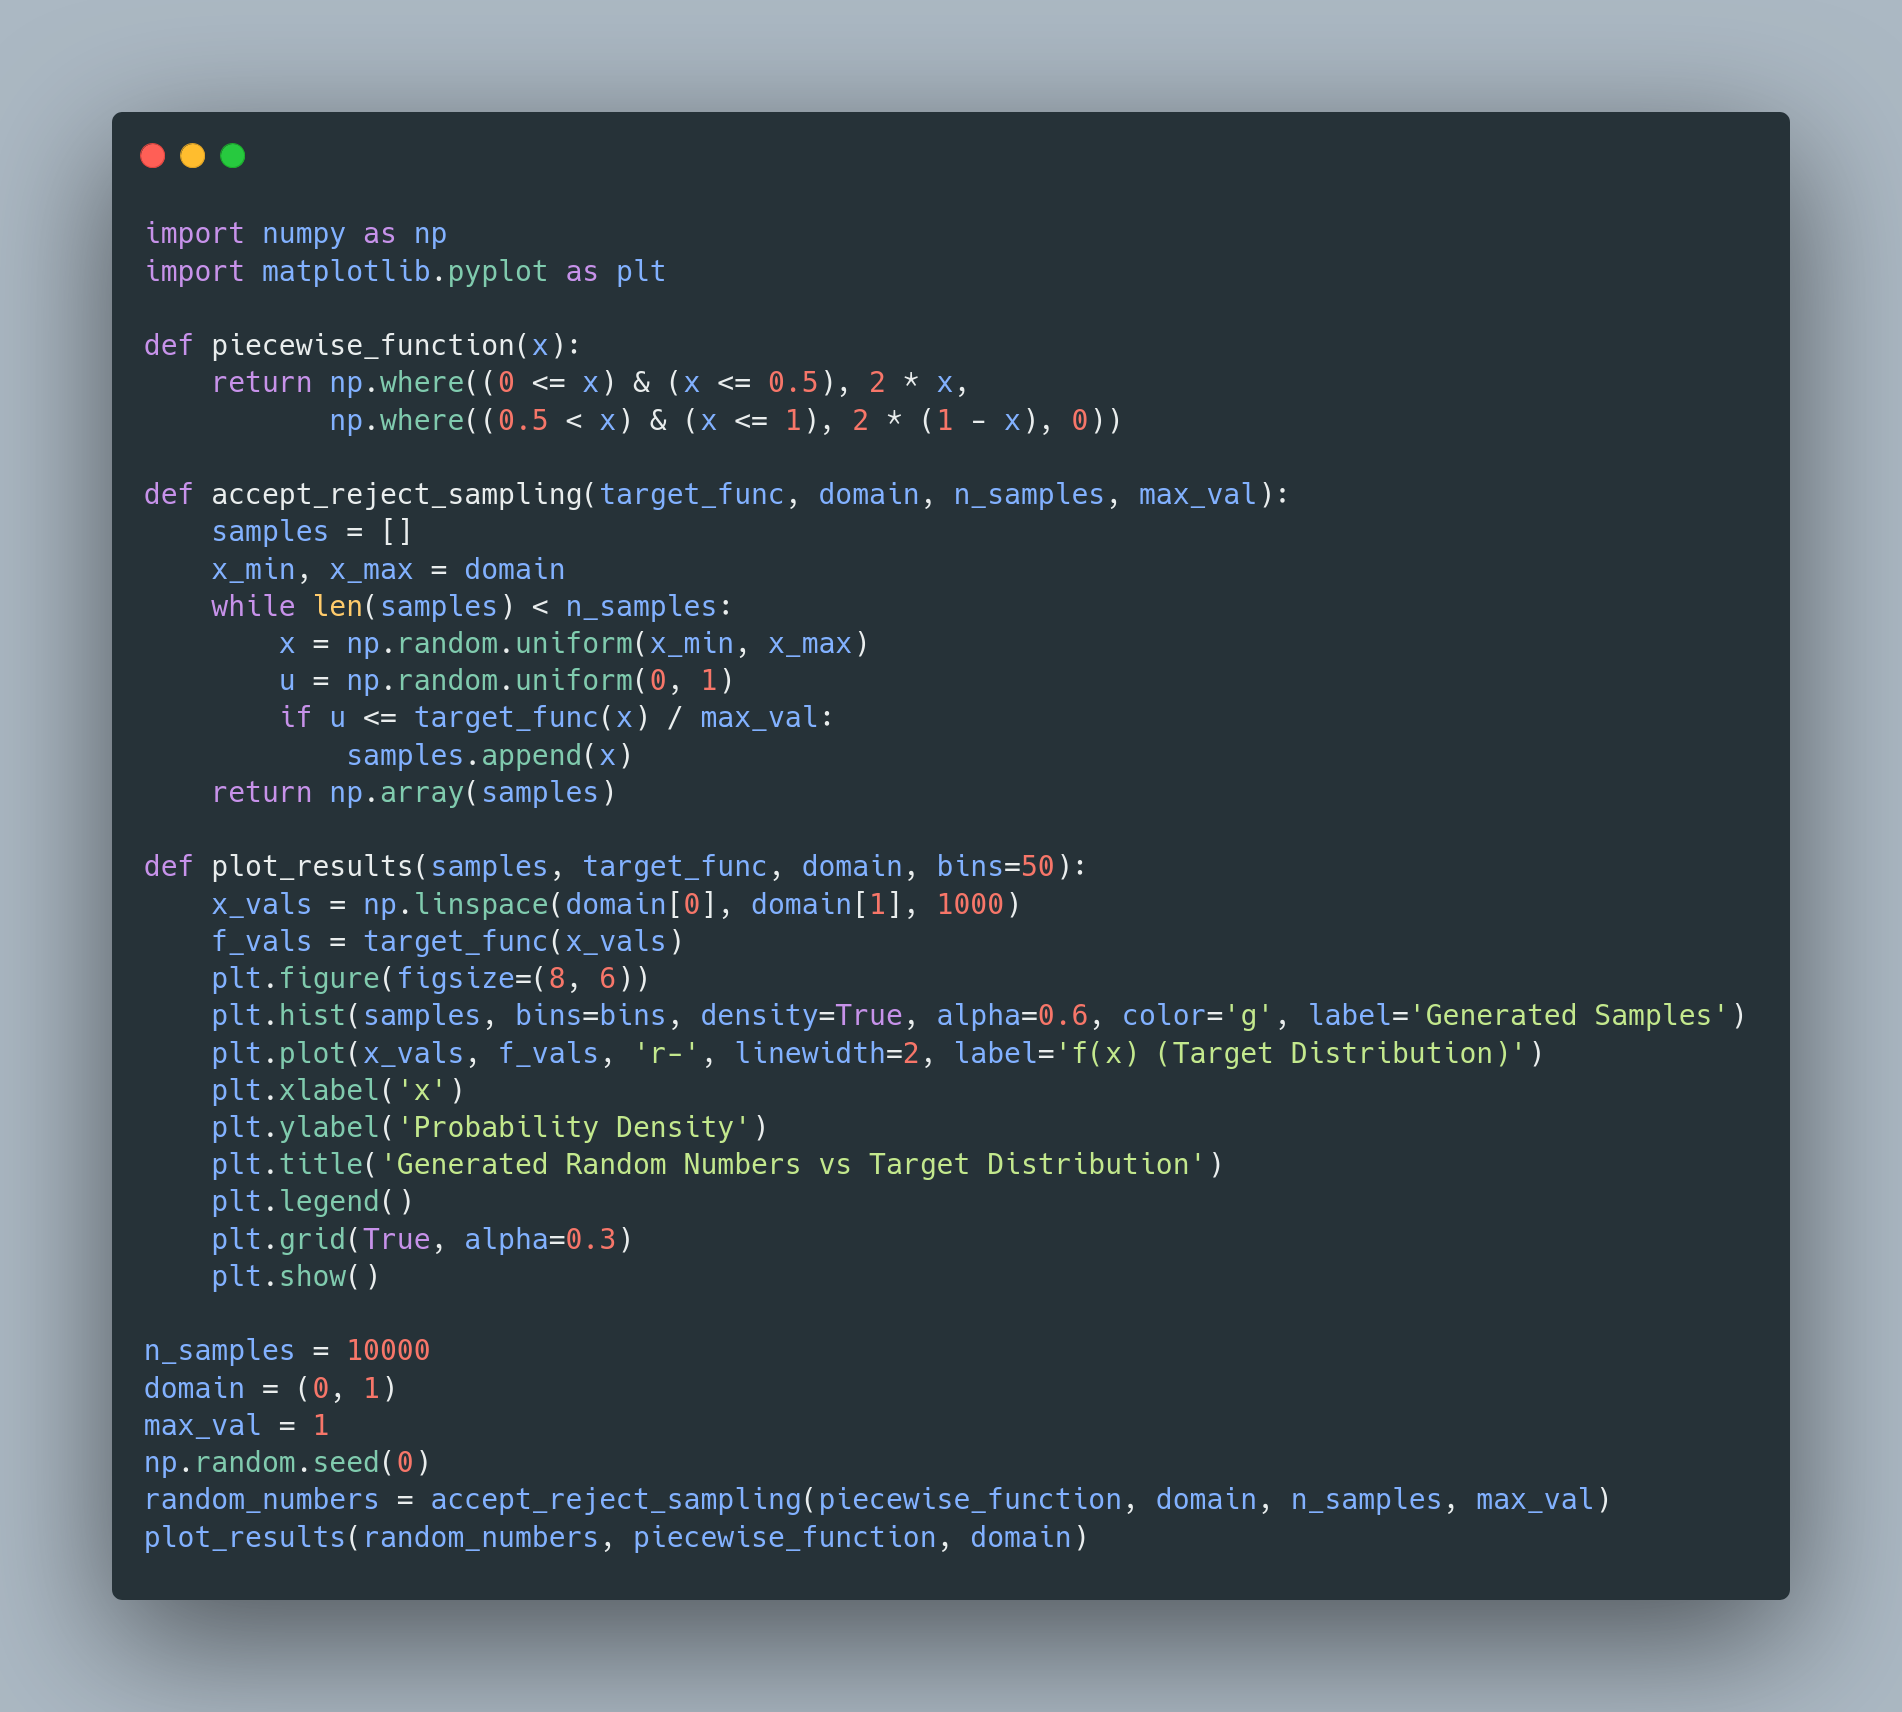
\includegraphics[width=0.6\textwidth]{./Screenshots/1.py.png} 
\end{figure} \\
\begin{figure}[h!]
    \centering
    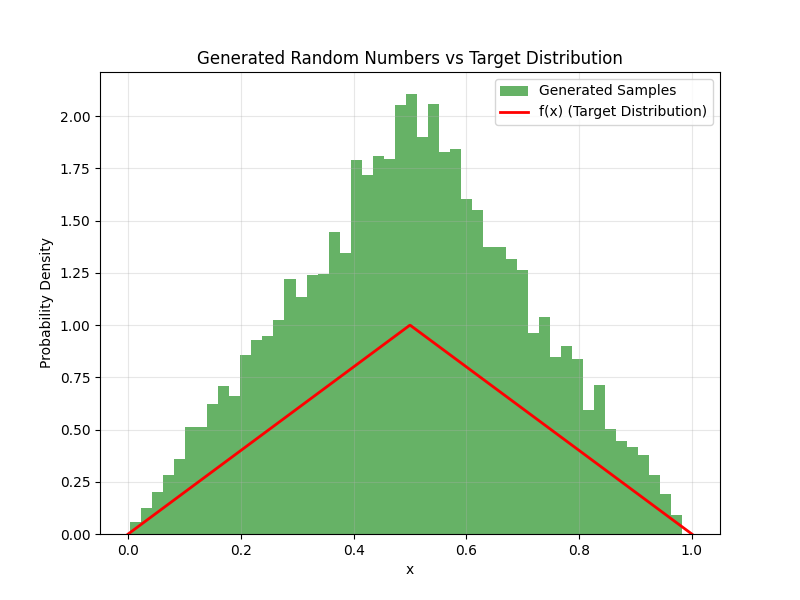
\includegraphics[width=0.6\textwidth]{./Screenshots/1.png} 
\end{figure} 
\newpage

\section{Exercise 2}
Simulate the distribution of angles at which particles scatter when the probability distribution of scattering angles is proportional to $\cos^2(x)$. Use the \textbf{accept-reject method} to generate the angles.
\begin{figure}[h!]
    \centering
    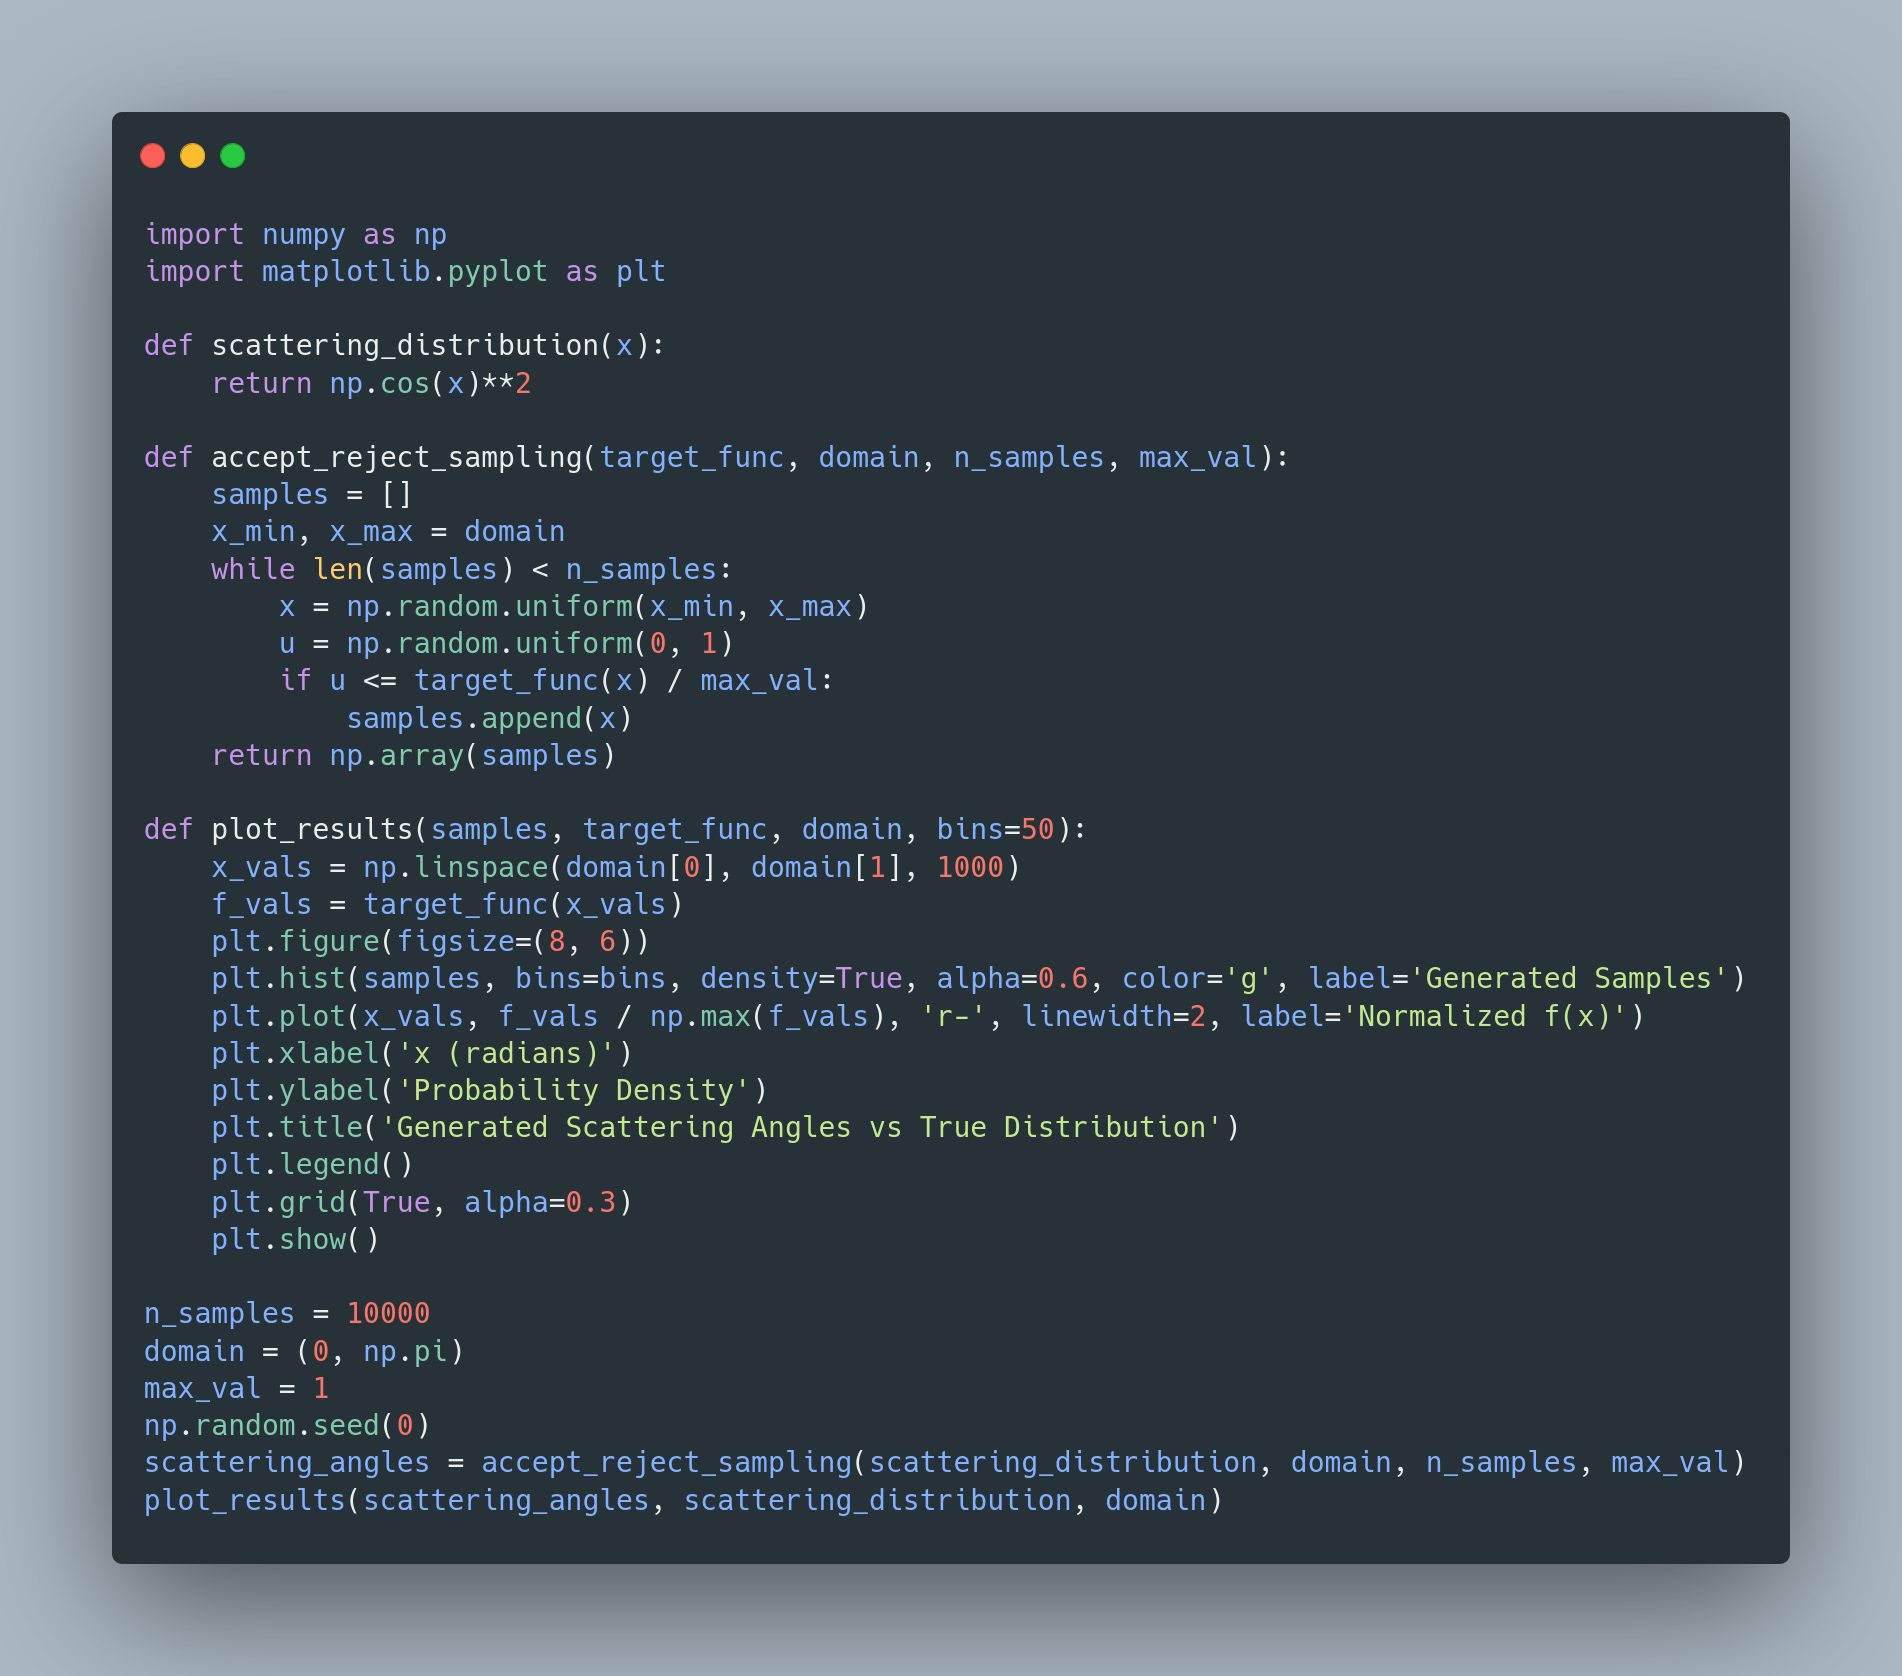
\includegraphics[width=0.6\textwidth]{./Screenshots/2.py.png} 
\end{figure} \\
\begin{figure}[h!]
    \centering
    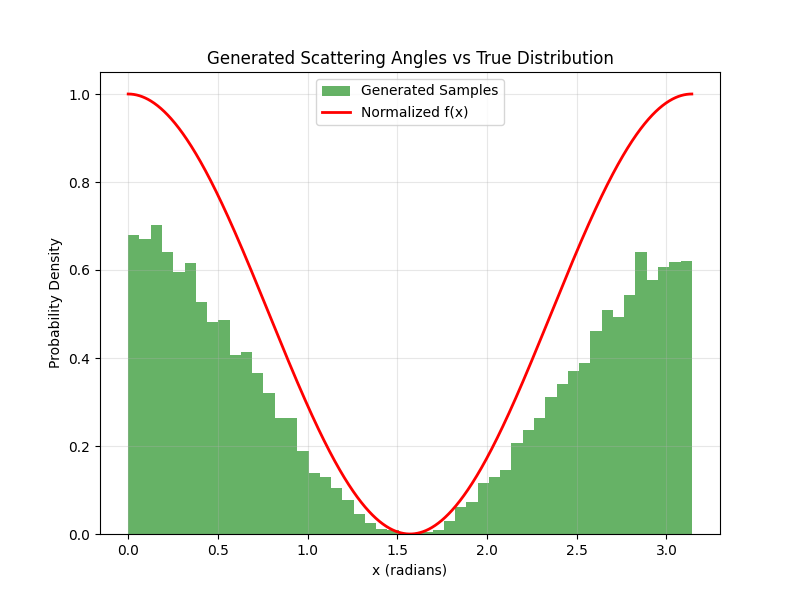
\includegraphics[width=0.6\textwidth]{./Screenshots/2.png} 
\end{figure} 
\newpage

\section{Exercise 3}
Simulate service times for customers in a queue. Assume service times follow a specific distribution (e.g., $f(x) = x e^{-x}$), and use the \textbf{accept-reject method} to generate the times. Analyze the average waiting time.
\begin{figure}[h!]
    \centering
    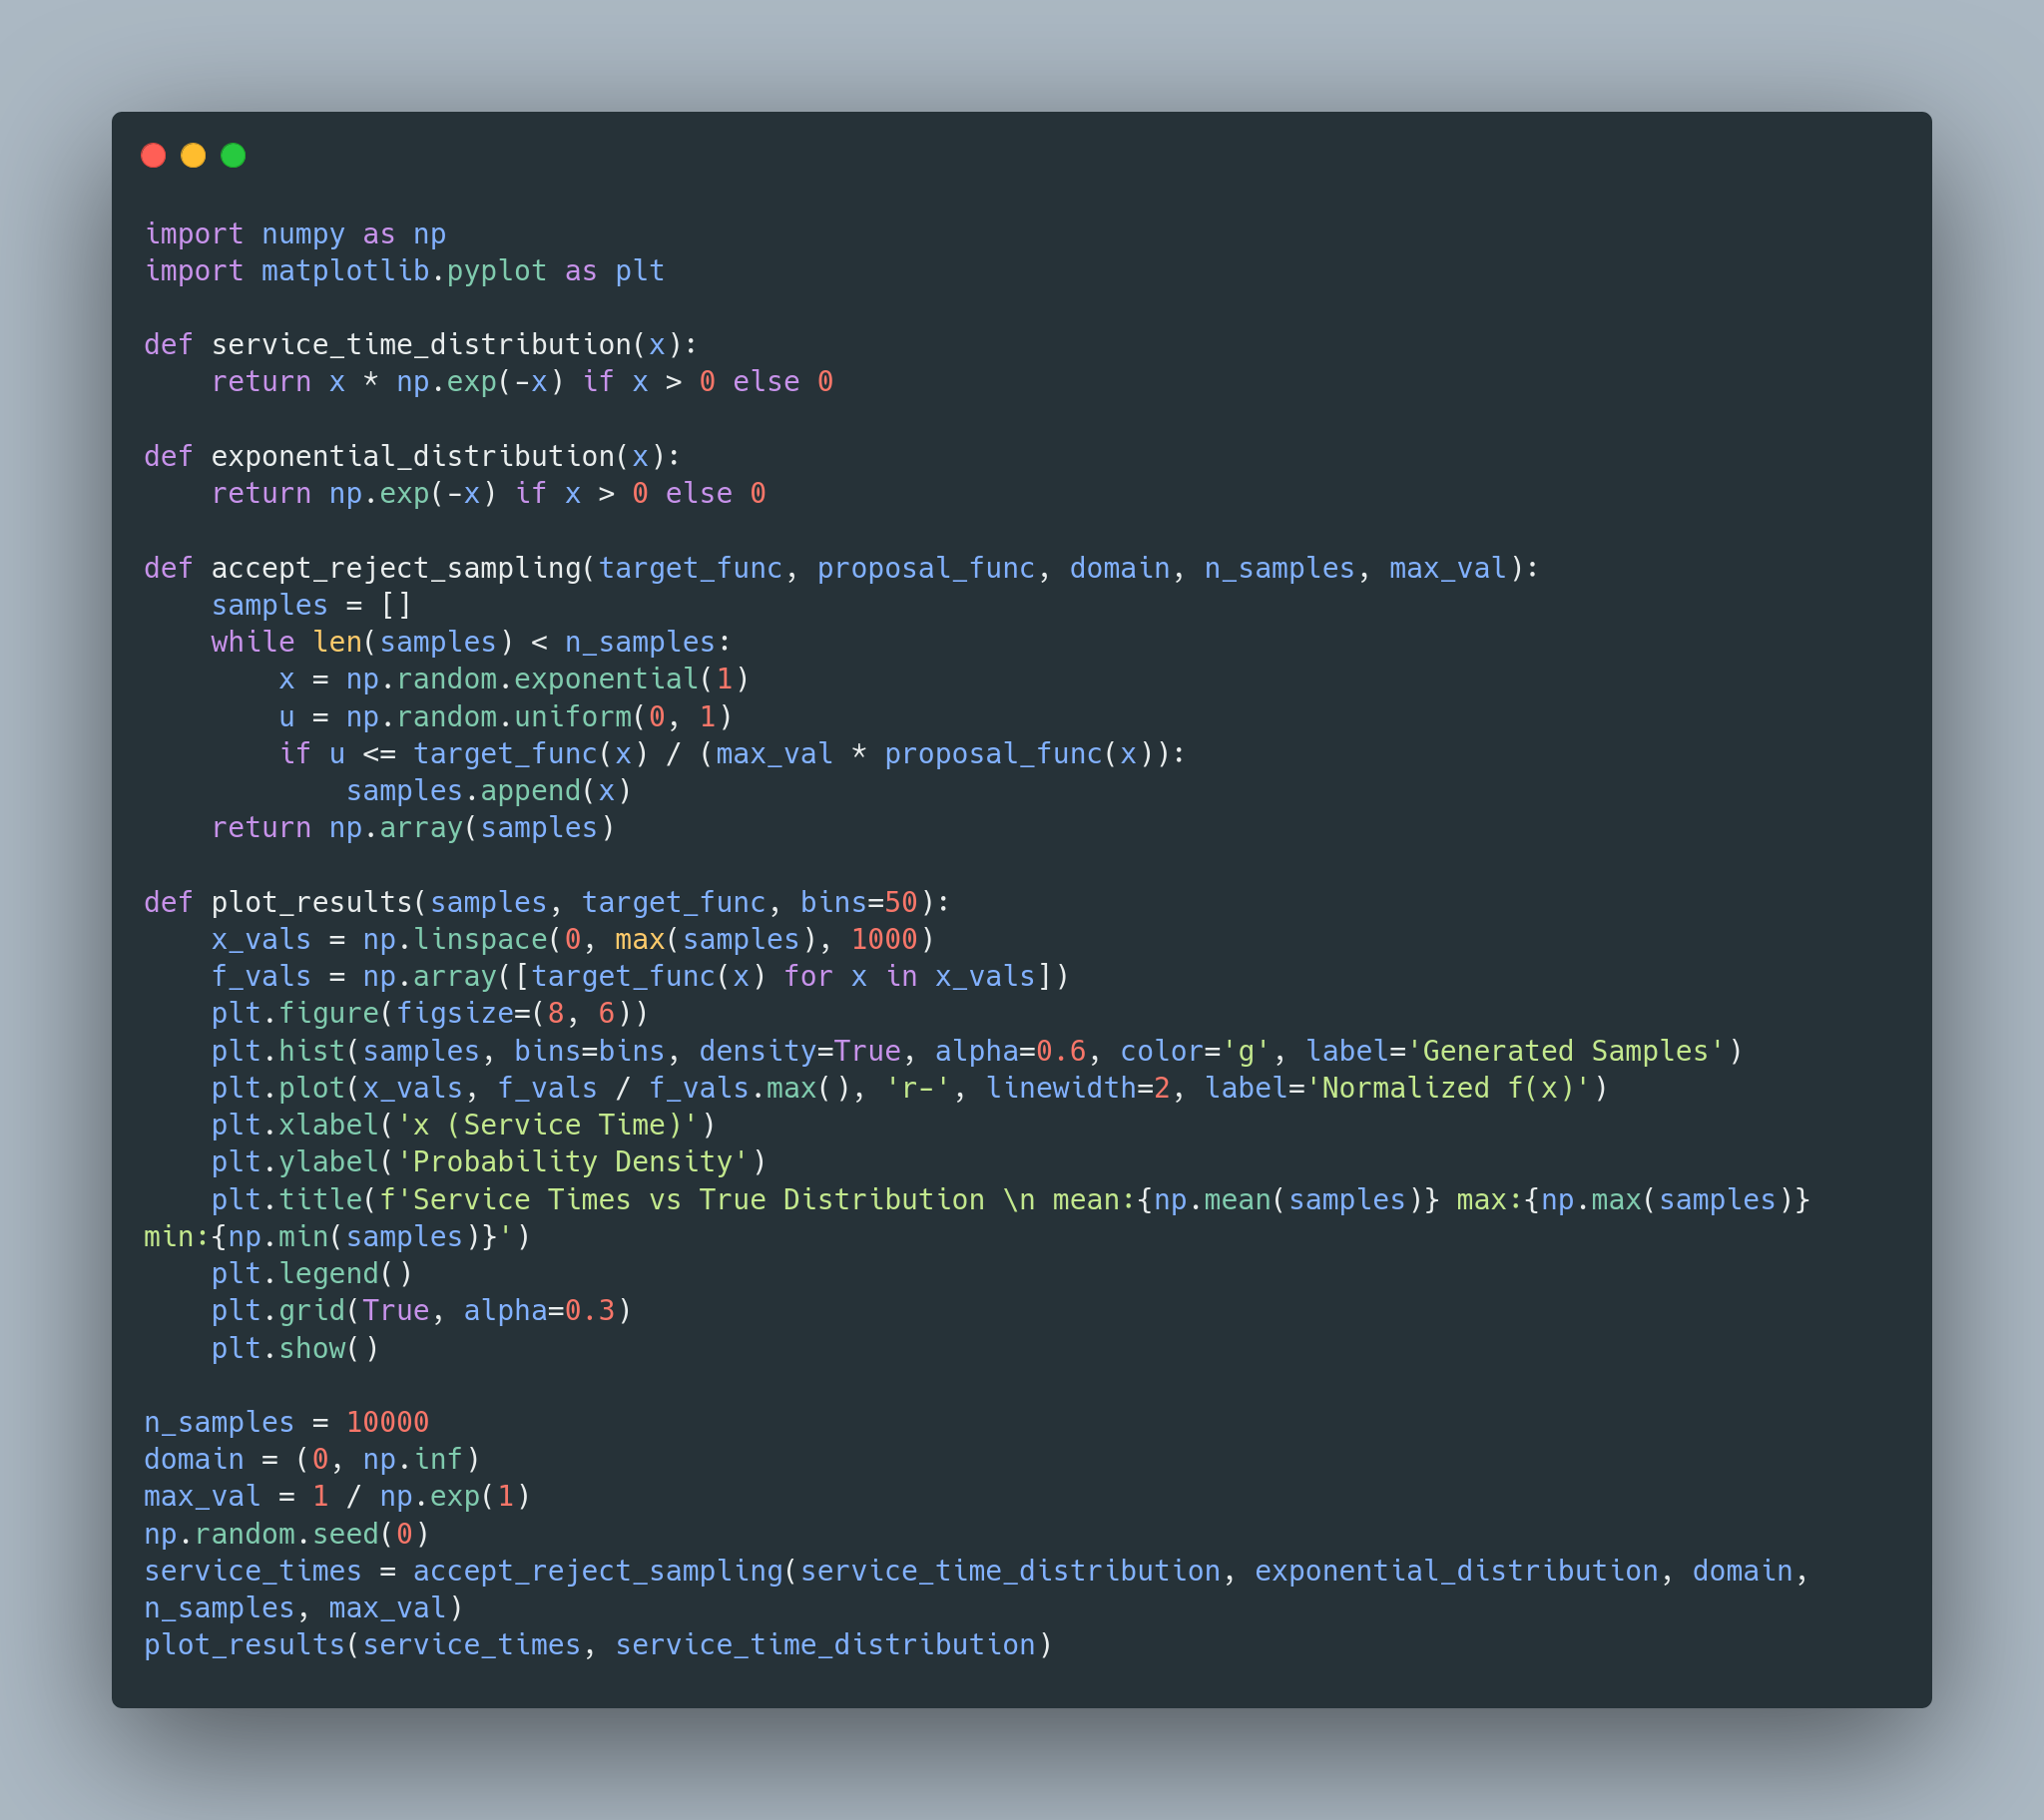
\includegraphics[width=0.6\textwidth]{./Screenshots/3.py.png} 
\end{figure} \\
\begin{figure}[h!]
    \centering
    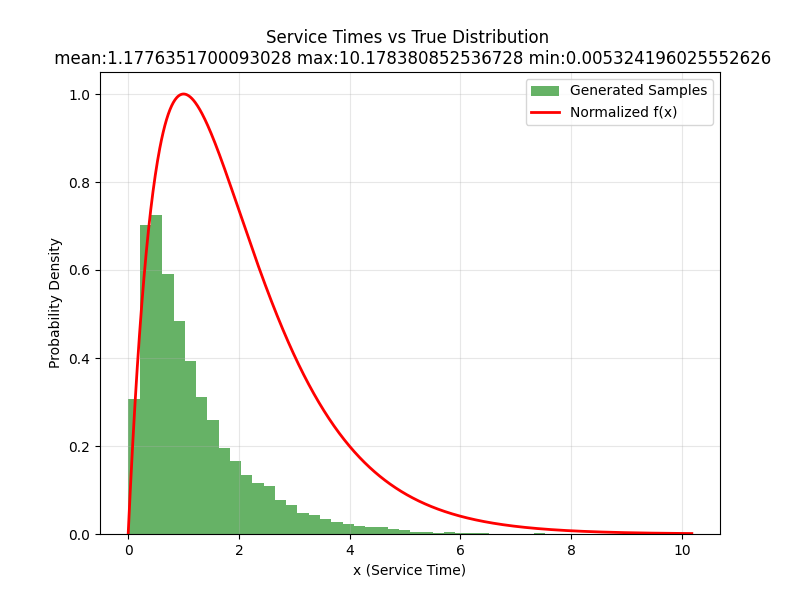
\includegraphics[width=0.6\textwidth]{./Screenshots/3.png} 
\end{figure} 
\newpage

\section{Exercise 4}
Generate random numbers for a triangular distribution defined on $[a, b]$ with mode $c$.
\begin{figure}[h!]
    \centering
    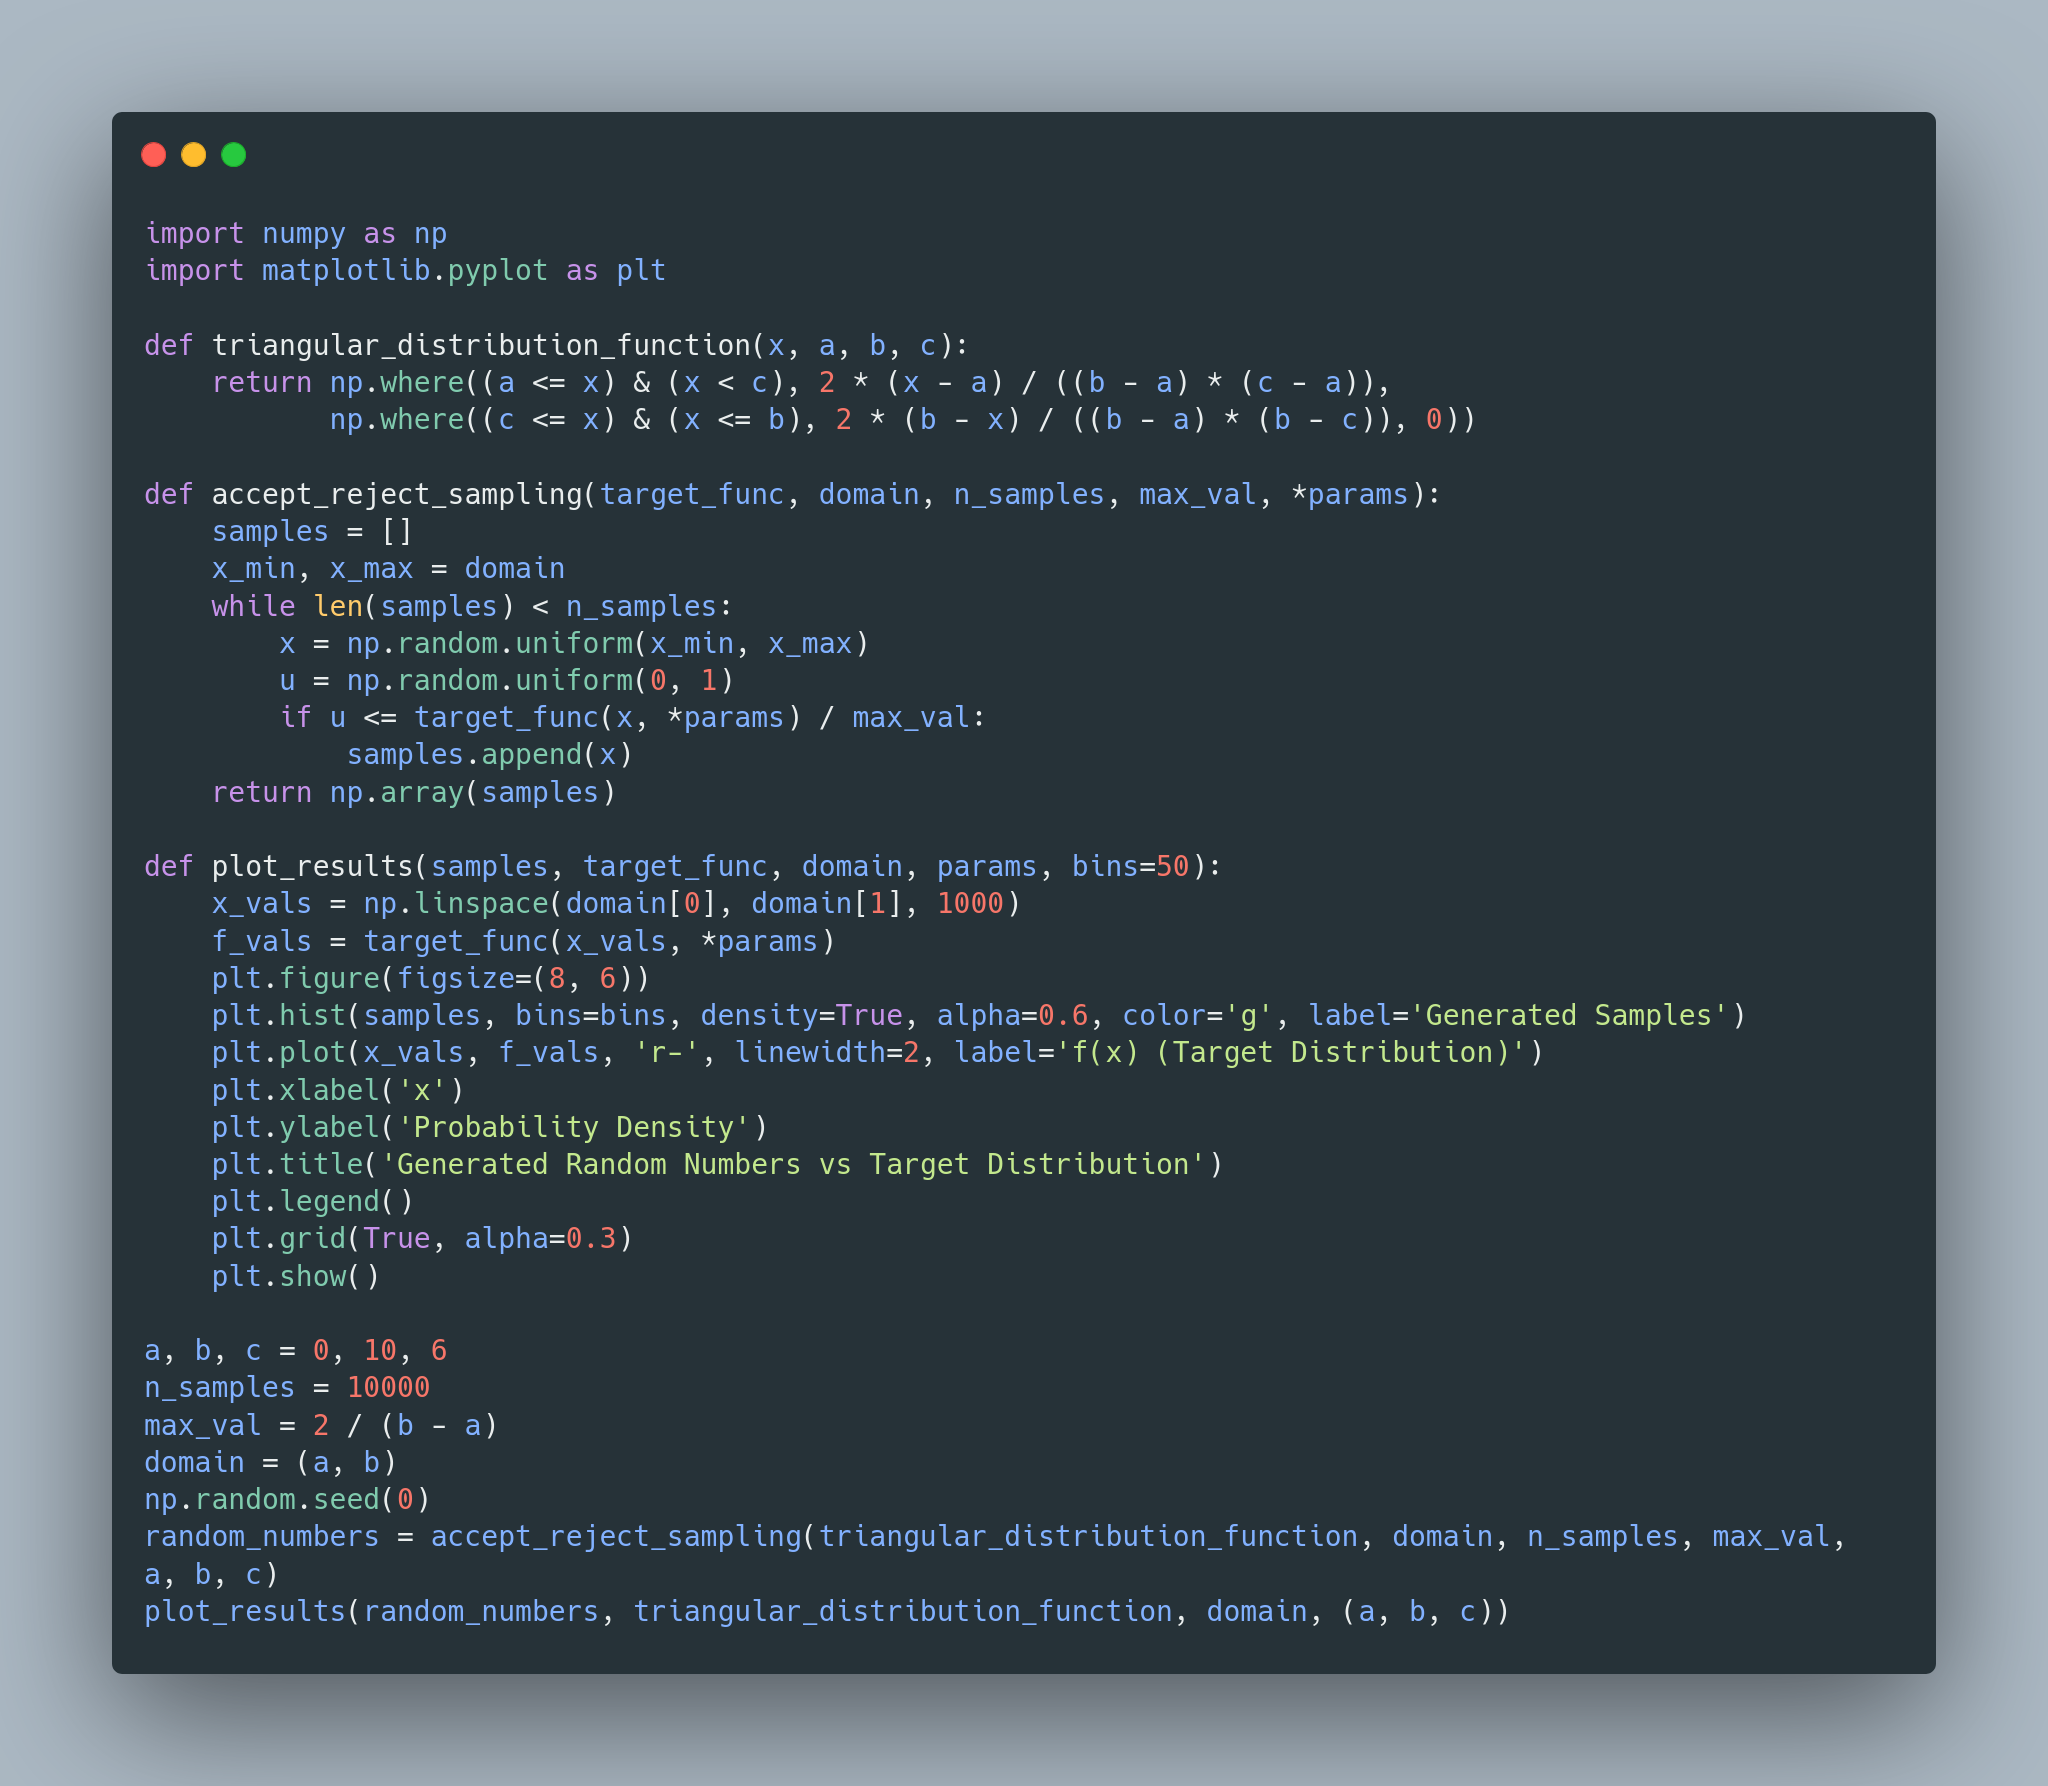
\includegraphics[width=0.6\textwidth]{./Screenshots/4.py.png} 
\end{figure} \\
\begin{figure}[h!]
    \centering
    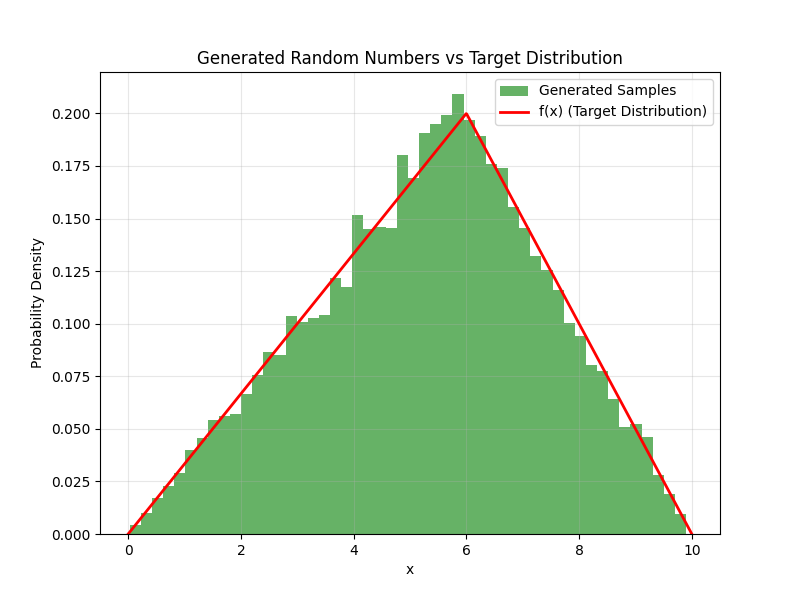
\includegraphics[width=0.6\textwidth]{./Screenshots/4.png} 
\end{figure} 
\newpage

\section{Exercise 5}
Implement a random number generator for the Rayleigh distribution with variance $\sigma^2$.

\section{Exercise 6}
Imagine a bank with multiple counters where customers arrive randomly. The arrival times of customers are independent and can be modeled using an exponential distribution. Similarly, the time taken to service a customer at a counter (service time) is also random and follows an exponential distribution.

\textbf{Tasks:}
\begin{itemize}
    \item Simulate customer arrivals and service times over a period.
    \item Analyze key metrics such as:
    \begin{itemize}
        \item Average waiting time,
        \item Counter utilization (how busy they are),
        \item Total time customers spend in the system.
    \end{itemize}
\end{itemize}

\section{Exercise 7}
A logistics company operates a fleet of drones to deliver packages. Each package has a random destination within a defined area, and each drone has constraints like maximum payload and battery range. Packages arrive randomly over time, and drones are dispatched accordingly.

\textbf{Inputs:}
\begin{itemize}
    \item Delivery area: A 2D space (e.g., a grid of $10 \times 10$ km).
    \item Drone characteristics: Speed, maximum payload, and battery range.
    \item Package data: Randomly generated delivery locations, weights, and arrival times.
\end{itemize}

\textbf{Tasks:}
\begin{enumerate}
    \item Generate random package data.
    \item Develop drone dispatch logic.
    \item Simulate drone movements.
    \item Analyze metrics such as:
    \begin{itemize}
        \item Average delivery time,
        \item Total distance traveled by all drones.
    \end{itemize}
\end{enumerate}
\end{document}
